The original implementation of \pygbe used continuum electrostatic theory to compute
the solvation energy of biomolecular systems. In that context, biomolecules were modeled as 
dielectric cavities inside an infinite continuum solvent, and the resulting partial differential
equations were solved using a boundary integral approach \cite{CooperBardhanBarba2013,CooperClementiBarba2015}.

The present work extends \pygbe to the LSPR biosensing application. Here, we write Maxwell's equations as a Laplace
equation, which is a valid approximation in the long-wavelength limit.
Modifications to \pygbe were required to allow for complex-valued permittivities, and to include the
effect of an external electric field.

\subsection{Scattering of small particles} \label{sec:scattering_small}

Electromagnetic scattering is usually modeled with Maxwell's equations.
However, when the wavelength of the incoming wave is much larger than the
scatterer, these can be reduced to a \emph{quasi-static} 
first-order approximation \cite{MayergoyzZhang2007}:
%
\begin{align} \label{eq:electrostatic_scatter_E}
\nabla \cdot \mathbf{E}_{1s} &= 0 \qquad \nabla \times \mathbf{E}_{1s} = 0, \nonumber \\
\nabla \cdot \mathbf{E}_{2s} &= 0 \qquad \nabla \times \mathbf{E}_{2s} = 0, \nonumber \\
\text{with interface conditions, } \nonumber \\
(\epsilon_1\mathbf{E}_{1s} - \epsilon_2\mathbf{E}_{2s})\cdot\mathbf{n} &= (\epsilon_2-\epsilon_1)\mathbf{E}_i\cdot \mathbf{n}.
\end{align}
%
In Equation \eqref{eq:electrostatic_scatter_E}, $\mathbf{E}_{1s}$ and $\mathbf{E}_{2s}$ 
are the electric fields of the scattered wave in the nanoparticle and host regions, respectively 
(see Figure \ref{fig:part_wave}), 
$\mathbf{E}_{i}$ is the field of the incoming wave, and $\epsilon_1$ 
and $\epsilon_2$ are the permittivities.
This approximation decouples the electric and magnetic fields, neglects the magnetic field, 
and describes the electric field as a curl-free vector field.
Hence, we can reformulate Equation \eqref{eq:electrostatic_scatter_E} with a scalar potential
($-\nabla \phi_{js} = \mathbf{E}_{js}$), as follows:
%
\begin{align} \label{eq:electrostatic_scatter}
\nabla^2 \phi_{1s} &= 0 \qquad \nabla^2 \phi_{2s} = 0 \qquad\text{on $\Omega_1$, $\Omega_2$} \nonumber \\
\epsilon_1\frac{\partial\phi_{1s}}{\partial \mathbf{n}} - \epsilon_2\frac{\partial\phi_{2s}}{\partial\mathbf{n}} &= (\epsilon_2-\epsilon_1)\frac{\partial\phi_i}{\partial\mathbf{n}} \quad \phi_{1s} = \phi_{2s} \quad \text{on $\Gamma$}.
\end{align}
%
Equation \eqref{eq:electrostatic_scatter} is an electrostatic equation 
with an imposed electric field $\mathbf{E}_i$.

\begin{figure}[h] %  figure placement: here, top, bottom, or page
   \centering
   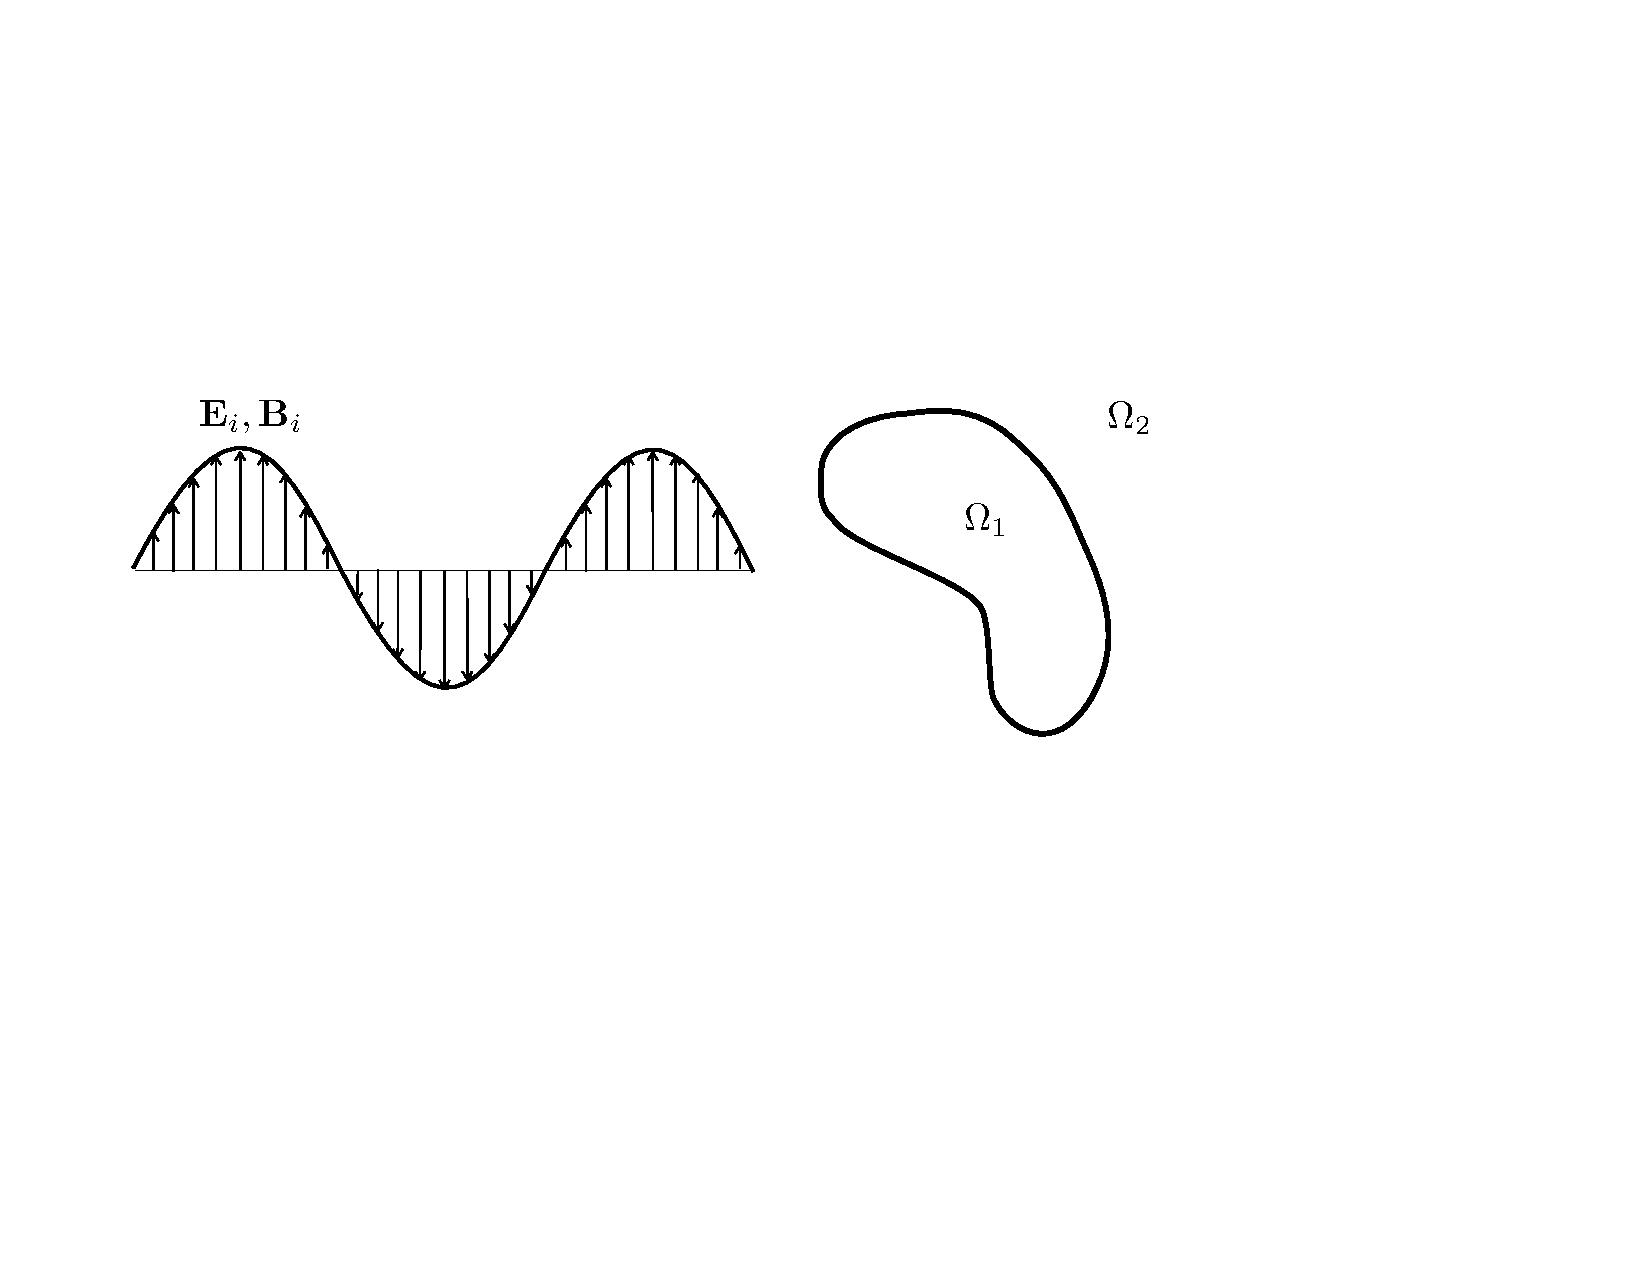
\includegraphics[width=0.45\textwidth]{particle_wave.pdf} 
   \caption{Nanoparticle under electromagnetic wave.}
   \label{fig:part_wave}
\end{figure}

\subsection{Far-field scattering} \label{sec:ff_scattering}

In LSPR, the scattered electromagnetic wave is measured by a detector located far away 
from the scatterer (nanoparticle), and plasmon resonance is identified when the energy 
detected is minimum. In the far-field limit, the scattered field
in the outside region ($\Omega_2$) is given by: 

\begin{equation} \label{eq:scat_efield_long_range}
    \mathbf{E}_{2s} = \frac{1}{4\pi\epsilon_2}k^2\frac{e^{ikr}}{r} (\mathbf{\hat{r}} \times \mathbf{p})\times\mathbf{\hat{r}}.
\end{equation} 

\noindent where $k=2\pi/\lambda$ is the wave number and $\lambda$ the wavelength, $\mathbf{\hat{r}}$ 
is a unit vector in the direction of the observation point, and $\mathbf{p}$ is
the dipole moment.
From a different approach, we can also obtain the scattered field using the 
scattering amplitude \cite{Jackson}:

\begin{equation} \label{eq:scat_efield_fwa}
    \mathbf{E}_{2s}(\mathbf{r})_{r\to\infty} = \frac{e^{ikr}}{r} \mathbf{F}(\mathbf{k},\mathbf{k}_0),
\end{equation}

\noindent where $\mathbf{F}$ is the scattering amplitude, $\mathbf{k}$ is the 
scattered wave vector in the direction of propagation, and $\mathbf{k}_0$ the 
wave vector of the incident field. 

\subsection{Extinction cross-section and Optical theorem} \label{sec:cext_ot}

The extinction cross-section ($C_\text{ext}$) is a measure of the energy that 
does not reach the detector, either because of scattering in other directions,
or absorption. This quantity is defined as the ratio of the lost energy and 
the intensity of the incoming wave, and has units of area. When there is 
resonance of plasmons, the extinction cross-section should peak.

On the other hand, the optical theorem relates the extinction cross-section with 
the forward-scattering amplitude. 
The traditional expression for this relationship applies for non-absorbing media 
\cite{MayergoyzZhang2007, Jackson}, however, it was corrected for absorbing media 
by Mishchenko \cite{Mishchenko2007}, giving the following expression:

\begin{equation} \label{eq:cext_fwa}
    C_\text{ext} = \frac{4\pi}{k^\prime} \operatorname{Im} \left[ \frac{\mathbf{\hat{e}}_i}{|\mathbf{E}_i|}\mathbf{F}(\mathbf{k}=\mathbf{k}_0, \mathbf{k}_0) \right].
\end{equation}


{\color{red}{Chris in Mishenko 2007 paper the equation is not exactly the same 
(look eq 87 in paper), do you have that derivation? How you got to the eq 7.22 
 in your thesis?.}\textcolor{blue}{I'll check this}}


Here, $k^\prime$ is the real part of the complex wave number. 

\begin{equation}
    k = k^\prime + ik^{\prime\prime} = \frac{2\pi}{\lambda} n,
\end{equation}

and $n$ is the refraction index of the host medium.

Combining Equations \eqref{eq:scat_efield_long_range} and \eqref{eq:scat_efield_fwa},
we can compute the scattering amplitude to then obtain the extinction cross-section 
with Equation \eqref{eq:cext_fwa}


\subsection{The boundary element method} \label{sec:lspr_bem}

\subsubsection{Electrostatic potential of a nanoparticle under an electric field} \label{sec:pot_elec_field}

\paragraph{Integral formulation}

Using Green's second identity, the system of partial differential equations 
in Equation \eqref{eq:electrostatic_scatter_E} can be rewritten as a system 
of boundary integral equations \cite{BrebbiaDominguez1992}. Evaluating on the surface $\Gamma$, this
becomes
%
\begin{align} \label{eq:integral_eq_lspr_nobc}
\frac{\phi_{1s,\Gamma}}{2}+ K_{L}^{\Gamma}(\phi_{1s,\Gamma}) - V_{L}^{\Gamma} \left(\frac{\partial}{\partial \mathbf{n}}\phi_{1s,\Gamma} \right) = 0&  \nonumber \\
\frac{\phi_{2s,\Gamma}}{2} - K_{L}^{\Gamma}(\phi_{2s,\Gamma}) + V_{L}^{\Gamma} \left( \frac{\partial}{\partial \mathbf{n}} \phi_{2s,\Gamma} \right) = 0&,
\end{align}
%
where $V$ and $K$ are the single and double layer operators, respectively:
%
\begin{equation}\label{eq:single_layer}
V^{\mathbf{r}_\Gamma}_L (\psi(\mathbf{r}_\Gamma)) = \oint_\Gamma \psi(\mathbf{r}'_\Gamma) G_L(\mathbf{r}_\Gamma, \mathbf{r}'_\Gamma) \text{d} \Gamma'.
\end{equation}

\begin{equation}\label{eq:double_layer}
K^{\mathbf{r}_\Gamma}_L (\psi(\mathbf{r}_\Gamma)) = \oint_\Gamma \psi(\mathbf{r}'_\Gamma) \frac{\partial}{\partial \mathbf{n}}G_L(\mathbf{r}_\Gamma, \mathbf{r}'_\Gamma) \text{d} \Gamma'.
\end{equation}
%

Here, $G_L$ is the free space Green's function of the Laplace equation
%
\begin{equation}
G_L(\mathbf{r},\mathbf{r}') = \frac{1}{4\pi|\mathbf{r}-\mathbf{r}'|}
\end{equation}

Applying the interface conditions of Equation \eqref{eq:electrostatic_scatter},
leads to:
%
\begin{align} \label{eq:integral_eq_lspr}
\frac{\phi_{1s,\Gamma}}{2}+ K_{L}^{\Gamma}(\phi_{1s,\Gamma}) - V_{L}^{\Gamma} \left(\frac{\partial}{\partial \mathbf{n}}\phi_{1s,\Gamma} \right) &= 0  \nonumber \\
\frac{\phi_{1s,\Gamma}}{2} - K_{L}^{\Gamma}(\phi_{1s,\Gamma}) + \frac{\epsilon_1}{\epsilon_2}V_{L}^{\Gamma} \left( \frac{\partial}{\partial \mathbf{n}} \phi_{1s,\Gamma}  \right) &= \frac{\epsilon_2-\epsilon_1}{\epsilon_2}V_{L}^{\Gamma}\left( \frac{\partial}{\partial \mathbf{n}} \phi_{i,\Gamma} \right)\quad \text{on $\Gamma$.}
\end{align}

%The weak formulation of Laplace equation with test function $w$:

%\begin{equation} \label{eq:lap_weak}
%\int_\Omega \nabla^2 \phi(\mathbf{r}_\Omega') w(\mathbf{r}_\Omega') \text{d} \Omega^\prime= 0.
%\end{equation}

%\noindent where the evaluation point is $\mathbf{r}_\Omega$ a location in the domain $\Omega$.

%If we use the Laplace's free-space Green's function as the test function $w$ we
%get:

%\begin{equation} \label{eq:lap_weak2}
%\int_\Omega \nabla^2 \phi(\mathbf{r}'_\Omega) G_L(\mathbf{r}_\Omega,\mathbf{r}'_\Omega) \text{d} \Omega^\prime= 0.
%\end{equation}

%Manipulating the integrand using the product rule and later the divergence 
%theorem, we get:

%\begin{equation} \label{eq:lap_bie_dom}
%\phi(\mathbf{r}_\Omega) = \oint_\Gamma G_L(\mathbf{r}_\Omega,\mathbf{r}'_\Gamma)  \frac{\partial} {\partial \mathbf{n}} \phi(\mathbf{r}'_\Gamma)  \text{d} \Gamma^\prime - \oint_\Gamma \phi(\mathbf{r}'_\Gamma)  \frac{\partial}{\partial \mathbf{n}} G_L(\mathbf{r}_\Omega,\mathbf{r}'_\Gamma) \text{d} \Gamma^\prime
%\end{equation}

%\noindent where \eqref{eq:lap_bie_dom}, $\mathbf{r}$ can be anywhere in the domain $\Omega$, 
%and $\mathbf{r}'$ runs only on the boundary $\Gamma$. This equation has a 
%singularity when $\mathbf{r}=\mathbf{r}'$. To handle this problem, we perform the
%integral on a surface $\Gamma'$ that is like $\Gamma$ but with a hemisphere of 
%radius $\varepsilon$ center at $\mathbf{r}$. We split the integrals into the part
%that we have no singularity and the part that has the hemisphere. After solving these
%equations when $\varepsilon \to 0$, equation \eqref{eq:lap_bie_dom} results in:

%\begin{equation} \label{eq:lap_bie}
%\frac{\phi(\mathbf{r}_\Gamma)}{2} +  \oint_\Gamma \phi(\mathbf{r}'_\Gamma)  \frac{\partial}{\partial \mathbf{n}} G_L(\mathbf{r}_\Gamma,\mathbf{r}'_\Gamma) \text{d} \Gamma^\prime = \oint_\Gamma G_L(\mathbf{r}_\Gamma,\mathbf{r}'_\Gamma)  \frac{\partial} {\partial \mathbf{n}} \phi(\mathbf{r}'_\Gamma)  \text{d} \Gamma^\prime,
%\end{equation}

%\noindent where these are Cauchy principal value integrals.

%Using the single and double layer operators:

%{\color{red} Chris, V is single layer operator but is it K the double layer one? 
%In your thesis you have that the double layer is W and you refers as K as
%"an operator" eq 2.108 and 2.112 in your thesis. Also shouldn't the $\text{d} \Gamma$
%be $\text{d} \Gamma'$? }

%\begin{equation}\label{eq:single_layer}
%V^{\mathbf{r}_\Gamma}_L (\psi(\mathbf{r}_\Gamma)) = \oint_\Gamma \psi(\mathbf{r}'_\Gamma) G_L(\mathbf{r}_\Gamma, \mathbf{r}'_\Gamma) \text{d} \Gamma.
%\end{equation}

%\begin{equation}\label{eq:double_layer}
%K^{\mathbf{r}_\Gamma}_L (\psi(\mathbf{r}_\Gamma)) = \oint_\Gamma \psi(\mathbf{r}'_\Gamma) \frac{\partial}{\partial \mathbf{n}}G_L(\mathbf{r}_\Gamma, \mathbf{r}'_\Gamma) \text{d} \Gamma.
%\end{equation}

%We can rewrite equation \eqref{eq:lap_bie} using the operator notation, as:

%\begin{equation} \label{eq:lap_operator}
%\left[ \frac{\mathbb{I}}{2} + K_L^{\mathbf{r}_\Gamma} \right] \left( \phi_\Gamma \right) = V_L^{\mathbf{r}_\Gamma} \left( \frac{\partial}{\partial \mathbf{n}} \phi_\Gamma \right),
%\end{equation}

%\noindent where $\mathbb{I}$ is the identity operator.

%Following the same steps, we can rewrite the Laplace equations in equation
%\eqref{eq:electrostatic_scatter} as:

%
%\begin{align} \label{eq:integral_eq_lspr_nobc}
%\frac{\phi_{1s,\Gamma}}{2}+ K_{L}^{\Gamma}(\phi_{1s,\Gamma}) - V_{L}^{\Gamma} \left(\frac{\partial}{\partial \mathbf{n}}\phi_{1s,\Gamma} \right) = 0&  \nonumber \\
%\frac{\phi_{2s,\Gamma}}{2} - K_{L}^{\Gamma}(\phi_{2s,\Gamma}) + V_{L}^{\Gamma} \left( \frac{\partial}{\partial \mathbf{n}} \phi_{2s,\Gamma} \right) = 0& \quad \text{on $\Gamma$,}
%\end{align}

%Applying the interface conditions of Equation \eqref{eq:electrostatic_scatter},
%we get:

%\begin{align} \label{eq:integral_eq_lspr}
%\frac{\phi_{1s,\Gamma}}{2}+ K_{L}^{\Gamma}(\phi_{1s,\Gamma}) - V_{L}^{\Gamma} \left(\frac{\partial}{\partial \mathbf{n}}\phi_{1s,\Gamma} \right) = 0&  \nonumber \\
%\frac{\phi_{1s,\Gamma}}{2} - K_{L}^{\Gamma}(\phi_{1s,\Gamma}) + \frac{1}{\epsilon_2}V_{L}^{\Gamma} \left( \epsilon_1 \frac{\partial}{\partial \mathbf{n}} \phi_{1s,\Gamma} - (\epsilon_2-\epsilon_1) \frac{\partial}{\partial \mathbf{n}} \phi_{i,\Gamma} \right) = 0& \quad \text{on $\Gamma$.}
%\end{align}

\subsubsection{Analyte-sensor electrostatic potential under an electric field}

\textcolor{blue}{Might be a good idea to put most of this seciton on a appendix, but we should discuss this}
The sketch in Figure \ref{fig:analyte-sensor} shows a metallic nanoparticle ($\Omega_1$) interacting with an analyte ($\Omega_3$), under an external electric field.
Mathematically, this can be modeled as
%
\begin{align} \label{eq:electrostatic_scatter_prot_sen}
\nabla^2 \phi_{1s} &= 0 \qquad \nabla^2 \phi_{2s} = 0 \qquad\text{on $\Omega_1$, $\Omega_2$} \nonumber\\
\nabla^2 \phi_{3s} &= \frac{1}{4\pi\epsilon_3} \sum_{k=0}^{N_q} \frac{q_k}{|\mathbf{r}_{\Omega_3} - \mathbf{r}_k|} \qquad\text{on $\Omega_3$} \nonumber \\
\epsilon_1\frac{\partial\phi_{1s}}{\partial \mathbf{n}} - \epsilon_2\frac{\partial\phi_{2s}}{\partial\mathbf{n}} &= (\epsilon_2-\epsilon_1)\frac{\partial\phi_i}{\partial\mathbf{n}} \quad \phi_{1s} = \phi_{2s} \quad \text{on $\Gamma_1$}. \nonumber\\
\epsilon_3\frac{\partial\phi_{3s}}{\partial \mathbf{n}} - \epsilon_2\frac{\partial\phi_{2s}}{\partial\mathbf{n}} &= (\epsilon_2-\epsilon_3)\frac{\partial\phi_i}{\partial\mathbf{n}} \quad \phi_{3s} = \phi_{2s} \quad \text{on $\Gamma_2$}.
\end{align}
%

\begin{figure}[h] %  figure placement: here, top, bottom, or page
    \centering
    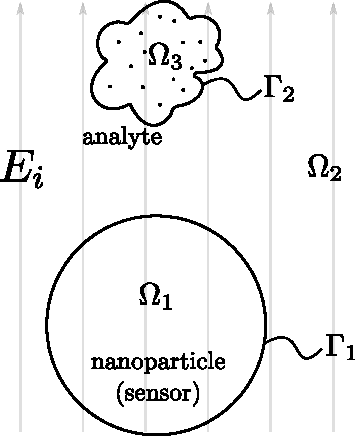
\includegraphics[width=0.20\textwidth]{protein_sensor_regions.pdf} 
    \caption{Analyte-sensor system under electric field.}
    \label{fig:analyte-sensor}
 \end{figure}

\paragraph{Integral formulation}

Similar to Equation \eqref{eq:integral_eq_lspr}, we can write the system of partial differential equations from \eqref{eq:electrostatic_scatter_prot_sen} as
%
\begin{align} \label{eq:integral_eq_lspr_nobc_system}
\frac{\phi_{1s,\Gamma_1}}{2}+ K_{L,\Gamma_1}^{\Gamma_1}(\phi_{1s,\Gamma_1}) - V_{L,\Gamma_1}^{\Gamma_1} \left(\frac{\partial}{\partial \mathbf{n}}\phi_{1s,\Gamma_1} \right) &= 0  \nonumber \\
\frac{\phi_{2s,\Gamma_1}}{2} - K_{L,\Gamma_1}^{\Gamma_1}(\phi_{2s,\Gamma_1}) + V_{L,\Gamma_1}^{\Gamma_1} \left(\frac{\partial}{\partial \mathbf{n}}\phi_{2s,\Gamma_1} \right) \nonumber\\
 - K_{L,\Gamma_2}^{\Gamma_1}(\phi_{2s,\Gamma_2}) + V_{L,\Gamma_2}^{\Gamma_1} \left(\frac{\partial}{\partial \mathbf{n}}\phi_{2s,\Gamma_2} \right) &= 0  \nonumber \\
\frac{\phi_{2s,\Gamma_2}}{2} - K_{L,\Gamma_1}^{\Gamma_2}(\phi_{2s,\Gamma_1}) + V_{L,\Gamma_1}^{\Gamma_2} \left(\frac{\partial}{\partial \mathbf{n}}\phi_{2s,\Gamma_1} \right) \nonumber \\ 
- K_{L,\Gamma_2}^{\Gamma_2}(\phi_{2s,\Gamma_2}) + V_{L,\Gamma_2}^{\Gamma_2} \left(\frac{\partial}{\partial \mathbf{n}}\phi_{2s,\Gamma_2} \right) &= 0  \nonumber \\
\frac{\phi_{3s,\Gamma_2}}{2} + K_{L,\Gamma_2}^{\Gamma_2}(\phi_{3s,\Gamma_2}) - V_{L,\Gamma_2}^{\Gamma_2} \left( \frac{\partial}{\partial \mathbf{n}} \phi_{3s,\Gamma_2} \right) &= \frac{1}{4\pi\epsilon_3} \sum_{k=0}^{N_q} \frac{q_k}{|\mathbf{r}_{\Gamma_2} - \mathbf{r}_k|} ,
\end{align}
%
Where $V$ and $K$ are the single and double layer operators from equations 
\eqref{eq:single_layer} and \eqref{eq:double_layer}. In this case, we distinct between the
surface where the integrals run (subindex), and the surface that contains the evaluation point (superindex).

Applying the interface condition of equation \eqref{eq:electrostatic_scatter_prot_sen},
leads to: 

\begin{align} \label{eq:integral_eq_lspr_nobc_system}
\frac{\phi_{1s,\Gamma_1}}{2}+ K_{L,\Gamma_1}^{\Gamma_1}(\phi_{1s,\Gamma_1}) - V_{L,\Gamma_1}^{\Gamma_1} \left(\frac{\partial}{\partial \mathbf{n}}\phi_{1s,\Gamma_1} \right) = 0 & \nonumber \\
\frac{\phi_{1s,\Gamma_1}}{2} - K_{L,\Gamma_1}^{\Gamma_1}(\phi_{1s,\Gamma_1}) + V_{L,\Gamma_1}^{\Gamma_1} \left(\frac{\epsilon_1}{\epsilon_2}\frac{\partial}{\partial \mathbf{n}}\phi_{1s,\Gamma_1} \right) - V_{L,\Gamma_1}^{\Gamma_1} \left(\frac{\epsilon_2-\epsilon_1}{\epsilon_2}\frac{\partial}{\partial \mathbf{n}}\phi_{i,\Gamma_1} \right) & \nonumber\\
 - K_{L,\Gamma_2}^{\Gamma_1}(\phi_{3s,\Gamma_2}) + V_{L,\Gamma_2}^{\Gamma_1} \left(\frac{\epsilon_3}{\epsilon_2}\frac{\partial}{\partial \mathbf{n}}\phi_{3s,\Gamma_2} \right)  - V_{L,\Gamma_2}^{\Gamma_1} \left(\frac{\epsilon_2 -\epsilon_3}{\epsilon_2}\frac{\partial}{\partial \mathbf{n}}\phi_{i,\Gamma_2} \right) = 0 &  \nonumber \\
\frac{\phi_{3s,\Gamma_1}}{2} - K_{L,\Gamma_1}^{\Gamma_2}(\phi_{1s,\Gamma_1}) + V_{L,\Gamma_1}^{\Gamma_2} \left(\frac{\epsilon_1}{\epsilon_2}\frac{\partial}{\partial \mathbf{n}}\phi_{1s,\Gamma_1} \right) - V_{L,\Gamma_1}^{\Gamma_2} \left(\frac{\epsilon_2-\epsilon_1}{\epsilon_2}\frac{\partial}{\partial \mathbf{n}}\phi_{i,\Gamma_1} \right) & \nonumber\\
 - K_{L,\Gamma_2}^{\Gamma_2}(\phi_{3s,\Gamma_2}) + V_{L,\Gamma_2}^{\Gamma_2} \left(\frac{\epsilon_3}{\epsilon_2}\frac{\partial}{\partial \mathbf{n}}\phi_{3s,\Gamma_2} \right)  - V_{L,\Gamma_2}^{\Gamma_2} \left(\frac{\epsilon_2 -\epsilon_3}{\epsilon_2}\frac{\partial}{\partial \mathbf{n}}\phi_{i,\Gamma_2} \right) = 0 &  \nonumber \\
\frac{\phi_{3s,\Gamma_2}}{2} + K_{L,\Gamma_2}^{\Gamma_2}(\phi_{3s,\Gamma_2}) - V_{L,\Gamma_2}^{\Gamma_2} \left( \frac{\partial}{\partial \mathbf{n}} \phi_{3s,\Gamma_2} \right) = \frac{1}{4\pi\epsilon_3} \sum_{k=0}^{N_q} \frac{q_k}{|\mathbf{r}_{\Gamma_2} - \mathbf{r}_k|} &
\end{align}


\paragraph{Discretization and linear system}

We discretize the surface into flat triangles, and assume that  $\phi$ and 
$\partial \phi/\partial \mathbf{n}$ are constant within each panel. Then, we can
write the layer operators in their discretized form:
%
\begin{align} \label{eq:layers_disc}
V_{L,\text{disc}}^{\mathbf{r}_\Gamma} \left( \frac{\partial}{\partial \mathbf{n}} \phi(\mathbf{r}_{\Gamma}) \right) &= \sum_{j=1}^{N_p} \frac{\partial}{\partial \mathbf{n}} \phi(\mathbf{r}_{\Gamma_j}) \int_{\Gamma_j} G_L(\mathbf{r}_\Gamma,\mathbf{r}_{\Gamma_j})  \mathrm{d} \Gamma_j  \nonumber \\
K_{L,\text{disc}}^{\mathbf{r}_\Gamma}(\phi(\mathbf{r}_{\Gamma})) &=  \sum_{j=1}^{N_p}\phi(\mathbf{r}_{\Gamma_j})\int_{\Gamma_j} \frac{\partial}{\partial \mathbf{n}} \left[ G_L(\mathbf{r}_\Gamma,\mathbf{r}_{\Gamma_j}) \right]\mathrm{d} \Gamma_j
\end{align}
%
\noindent where $N_p$ is the number of discretization elements on $\Gamma$, 
and $\phi(\mathbf{r}_{\Gamma_j})$ and $\frac{\partial}{\partial \mathbf{n}} 
\phi(\mathbf{r}_{\Gamma_j})$ are the values of $\phi$ and 
$\frac{\partial \phi}{\partial \mathbf{n}}$ on panel $\Gamma_j$.
Then, using centroid collocation, we can write equation \eqref{eq:integral_eq_lspr} in matrix form as:
%
 \begin{equation} \label{eq:matrix_lspr}
 \left[
    \begin{matrix} 
       \frac{1}{2} + K_{L}^{\Gamma} & -V_{L}^{\Gamma}  \vspace{0.2cm} \\
       \frac{1}{2} - K_{L}^{\Gamma} &  \frac{\epsilon_1}{\epsilon_2} V_{L}^{\Gamma}  \vspace{0.2cm} 
    \end{matrix}
    \right] \left[ 
    \begin{matrix} 
       \phi_{1s,\Gamma} \vspace{0.2cm} \\
       \frac{\partial}{\partial \mathbf{n}} \phi_{1s,\Gamma} \vspace{0.2cm}
    \end{matrix} 
     \right] =   
    \left[
    \begin{matrix} 
       0 \\
       V_{L}^{\Gamma} \left(\frac{\epsilon_2-\epsilon_1}{\epsilon_2}\right) \frac{\partial\phi_i}{\partial\mathbf{n}} \vspace{0.2cm} 
    \end{matrix}
    \right]
 \end{equation}
%
Also, Equation \eqref{eq:integral_eq_lspr_nobc_system} can be represented as:
%
\begin{align} \label{eq:matrix_multi}
 \left[
    \begin{matrix} 
       \frac{1}{2}+K_{L, \Gamma_1}^{\Gamma_1} & -V_{L, \Gamma_1}^{\Gamma_1} & 0 &  0   \vspace{0.2cm} \\
       \frac{1}{2}-K_{L, \Gamma_1}^{\Gamma_1} & \frac{\epsilon_1}{\epsilon_2} V_{L, \Gamma_1}^{\Gamma_1} & -K_{L, \Gamma_2}^{\Gamma_1} & \frac{\epsilon_3}{\epsilon_2} V_{L, \Gamma_2}^{\Gamma_1} \vspace{0.2cm}  \\
        -K_{L, \Gamma_1}^{\Gamma_2}&\frac{\epsilon_1}{\epsilon_2} V_{L, \Gamma_1}^{\Gamma_2} & \frac{1}{2}-K_{L, \Gamma_2}^{\Gamma_2}  &  \frac{\epsilon_3}{\epsilon_2} V_{L, \Gamma_2}^{\Gamma_2} \vspace{0.2cm} \\
       0 & 0 & \frac{1}{2}+K_{L, \Gamma_2}^{\Gamma_2}&  - V_{L, \Gamma_2}^{\Gamma_2}   \vspace{0.2cm} \\
    \end{matrix}
    \right] 
\cdot
 \left[
    \begin{matrix}
    \phi_{1,\Gamma_1} \vspace{0.2cm} \\
    \frac{\partial}{\partial \mathbf{n}} \phi_{1,\Gamma_1} \vspace{0.2cm} \\
    \phi_{3,\Gamma_2} \vspace{0.2cm} \\
    \frac{\partial}{\partial \mathbf{n}} \phi_{3,\Gamma_2} \vspace{0.2cm} \\
    \end{matrix}
\right]&
 \nonumber \\
 = \left[
    \begin{matrix}
    0 \vspace{0.2cm} \\
    V_{L,\Gamma_1}^{\Gamma_1} \left(\frac{\epsilon_2-\epsilon_1}{\epsilon_2}\frac{\partial}{\partial \mathbf{n}}\phi_{i,\Gamma_1} \right)
    + V_{L,\Gamma_2}^{\Gamma_1} \left(\frac{\epsilon_2 -\epsilon_3}{\epsilon_2}\frac{\partial}{\partial \mathbf{n}}\phi_{i,\Gamma_2} \right)
    \vspace{0.2cm}\\
    V_{L,\Gamma_1}^{\Gamma_2} \left(\frac{\epsilon_2-\epsilon_1}{\epsilon_2}\frac{\partial}{\partial \mathbf{n}}\phi_{i,\Gamma_1} \right)
    + V_{L,\Gamma_2}^{\Gamma_2} \left(\frac{\epsilon_2 -\epsilon_3}{\epsilon_2}\frac{\partial}{\partial \mathbf{n}}\phi_{i,\Gamma_2} \right)
    \vspace{0.2cm}\\
    \frac{1}{4\pi\epsilon_3}\sum_{k=0}^{N_q} \frac{q_k}{|\mathbf{r}_{\Gamma_2} - \mathbf{r}_k|} \vspace{0.2cm}  \\
    \end{matrix}
\right]&
\end{align}
%
\noindent where the elements of the matrix are
%
\begin{align} \label{eq:layers_element}
V_{L,ij}^{\Gamma} &= \int_{\Gamma_j} G_L(\mathbf{r}_{\Gamma_i},\mathbf{r}_{\Gamma_j})  \mathrm{d} \Gamma_j \nonumber \\
K_{L,ij}^{\Gamma} &= \int_{\Gamma_j} \frac{\partial}{\partial \mathbf{n}} \left[ G_L(\mathbf{r}_{\Gamma_i},\mathbf{r}_{\Gamma_j}) \right]\mathrm{d} \Gamma_j
\end{align}
%
\noindent with $\mathbf{r}_{\Gamma_i}$ being at the center of panel $\Gamma_i$.


\paragraph{Integral evaluation}

We evaluate the integrals in Equation \eqref{eq:layers_element} with Gauss quadrature
rules. However, the $1/r$ singularity of the Green's function is a
problem to obtain good accuracy when the integral is 
singular or near-singular. Therefore, we define three different regions:

\emph{Singular integrals:} If the collocation point is in the integrated panel,
there is a singularity that is difficult to resolve with standard
Gauss integration schemes. In this case, we use a semi-analytical technique 
\cite{HessSmith1967,ZhuHuangSongWhite2001} that places $N_k$ quadrature nodes on the 
edges of the triangle.

\emph{Near-singular integrals:} If the collocation point is close to the integration panel,
the integrand has a high gradient, and high-order quadrature rules are required. 
We use the representative length of the integrated triangle ($L = \sqrt{2\cdot\text{Area}}$)
to define a threshold of the \emph{close-by} region, for example, when the integration panel 
is $2L$ or less away from the collocation point. For near-singular integrals, we use 
$K_{fine}=19, 25 \; or \; 37$ points per triangle. 

\emph{Far-away integrals:} When the distance between the collocation point and the integration
panel is beyond the threshold, they are considered to be far-away. 
At this point, the integrand is smooth enough that we obtain good 
accuracy with low order integration, for example, with 
$K=1, 3 \; or \; 4$ Gauss quadrature points per boundary element. 

\subsubsection{Boundary integral expression of the dipole moment}

As shown in Equation \eqref{eq:scat_efield_long_range}, the scattered electric 
field in the far-away limit depends on the dipole moment. The dipole moment is 
defined as 
%
\begin{equation} \label{eq:dipole_def}
\mathbf{p} = \int_\Omega \mathbf{r} \rho \text{d}\Omega,
\end{equation}
%
and rewriting this equation using Gauss's law we obtain
%
\begin{equation} \label{eq:dipole_def_gauss}
\mathbf{p} = -\epsilon_2\int_\Omega \mathbf{r} \nabla^2 \phi_{2s} \text{d}\Omega.
\end{equation}
%
For component $i$, this becomes:
%
\begin{equation} \label{eq:dipole_def_gauss_i}
{p_i} = -\epsilon_2\int_\Omega {x_i} \nabla^2 \phi_{2s} \text{d}\Omega.
\end{equation}
%
From the identity
%
\begin{equation} \label{eq:identity_grad}
\nabla \cdot \left(f \mathbf{v}\right) = \left( \nabla f \right)\cdot \mathbf{v} + f\left(\nabla \cdot \mathbf{v}\right)
\end{equation}
%
with $f=x_i$ and $\mathbf{v} = \nabla\phi_{2s}$, we can rewrite Equation \eqref{eq:dipole_def_gauss_i}
as 
%
\begin{align} \label{eq:dip_gauss_interm_1}
- \frac{\mathbf{p_i}}{\epsilon_2} &= \int_\Omega \nabla \cdot \left( x_i \nabla \phi_{2s} \right) \; \text{d}\Omega - \int_\Omega \nabla x_i \cdot \nabla\phi_{2s} \; \text{d}\Omega \nonumber \\
&\text{and applying the divergence theorem} \nonumber \\
&= \oint_\Gamma  x_i  \nabla \phi_{2s} \cdot \mathbf{n} \; \text{d}\Gamma - \int_\Omega \nabla x_i \cdot \nabla\phi_{2s} \; \text{d}\Omega
\end{align}
%
Again, using the identity \eqref{eq:identity_grad} in Equation \eqref{eq:dip_gauss_interm_1}, this time, 
taking $f=\phi_{2s}$ and $\mathbf{v} = \nabla x_i$ we get:
%
\begin{align} \label{eq:dip_gauss_interm_2}
 &= \oint_\Gamma  x_i  \frac{\partial \phi_{2s}}{\partial n} \text{d}\Gamma - \left[ \int_\Omega \nabla \cdot \left( \phi_{2s} \nabla x_i \right)\;\text{d}\Omega - \int_\Omega  \phi_{2s} \nabla^2 x_i \;\text{d}\Omega\right] \nonumber\\
&\text{and applying the divergence theorem} \nonumber \\
&= \oint_\Gamma  x_i  \frac{\partial \phi_{2s}}{\partial n} \; \text{d}\Gamma - \oint_\Gamma \phi_{2s} \nabla x_i \cdot \mathbf{n} \; \text{d}\Gamma \nonumber \\
&= \oint_\Gamma  x_i  \frac{\partial \phi_{2s}}{\partial n} \; \text{d}\Gamma - \oint_\Gamma \phi_{2s} n_i \;\text{d}\Gamma
\end{align}
%
Along this derivation, the normals are pointing into $\Omega_1$. However, in our implementation 
all normals are pointing outwards, and we need to include an extra negative sign, yielding:
%
\begin{equation} \label{eq:dipole_def_gauss_i_final}
{p_i} = \epsilon_2 \left[ \oint_\Gamma  x_i  \frac{\partial \phi_{2s}}{\partial n} \text{d}\Gamma - \oint_\Gamma \phi_{2s} n_i \; \text{d}\Gamma \right].
\end{equation}

Using BEM, we obtain the electrostatic potential on the surface of the nanoparticle, 
which we use in Equation \eqref{eq:dipole_def_gauss_i_final} to get the dipole 
moment, and in Equation \eqref{eq:scat_efield_long_range} to obtain the scattered
electric field. From there, we can use Equation \eqref{eq:scat_efield_fwa} and Equation 
\eqref{eq:cext_fwa} to get the extinction cross section.

\subsection{Acceleration strategies} \label{sec:acc_strategies}

The main downside of the Boundary Element Method (\bem) is that it generates dense matrices
after discretization. Solving the linear system using
Gaussian elimination requires $\O{N^3}$ computations and $\O{N^2}$ storage, whereas for a
Krylov-subspace iterative solver, like the Generalized Minimal Residual Method (\gmres),
computations drop to $\O{N^2}$ because they are dominated by a matrix-vector 
product. This makes \bem a good approach for problems with no more than a few thousand boundary elements,
which is far from the mesh sizes required for real applications. 

Since we are using Gaussian quadrature and collocation, the matrix-vector product
becomes an N-body problem, where the Gauss nodes act as centers of mass (\emph{sources}), and we evaluate
the potential at the collocation points (\emph{targets}).
To overcome the $\O{N^2}$ scaling,
we accelerate the matrix-vector product using a Treecode algorithm \cite{BarnesHut1986,DuanKrasny2001}, 
which is a fast-summation algorithm capable of reducing $\O{N^2}$
computational patterns 
%
\begin{equation} \label{eq:summation}
V(\mathbf{x}_i) = \sum_{j=1}^{N} q_j \psi(\mathbf{x}_i, \mathbf{y}_j) 
\end{equation}
%
\noindent to a computational complexity of $\O{N \log N}$. In Equation \eqref{eq:summation} 
$q_j$ is the weight, $\psi$ the kernel, $\mathbf{y}_j$ the locations of sources and 
$\mathbf{x}_i$ the locations of targets.

The Treecode groups sources geometrically in boxes of an octree, which is built making
sure that no box in the lowest level has more than $N_\text{crit}$ sources. Then, if a group of
sources is far away from a target, their influence is aggregated in an expansion center,
and the target interacts with the box, rather than with each source independently.
On the other hand, if the group of targets is too close, the Treecode queries the child
boxes. If the box has no children and still is not far enough, the interaction is 
performed directly. The threshold to decide if a box is far enough is called the multipole-
acceptance criterion (MAC):
%
\begin{equation}
\theta > \frac{r_b}{r},
\end{equation}
%
where $r_b$ is the box size and $r$ the distance between the box center and the target.
Common values of $\theta$ are $1/2$ and $2/3$.
To approximate the contribution of the sources, we use Taylor expansions
of order $P$.
The Treecode allows us to control accuracy of the approximation by modifying $\theta$ and $P$.
Further details of the Treecode implementation in \pygbe can be found in \cite{CooperBarba-share154331,CooperBardhanBarba2013}.

\subsection{Code implementation details} \label{sec:code_imp}

As we mentioned at the beginning of this section, the original \pygbe code was 
adapted to suit the needs of the nano-plasmonic implementation. The main changes
were:

\begin{itemize}
    \item Re-write of the Generalized minimal residual method (GMRES) to accept complex numbers. 
    \item Split Treecode calculations into real and imaginary part.
    \item New format of config file that includes electric field intensity and  wavelength.
    \item Functions added:
    \subitem $read\_electric\_field$ : Reads the electric field intensity and its wavelength from config files.
    \subitem $dipole\_moment$ : Computes numerically the dipole moment (Eq. \eqref{eq:dipole_def_gauss_i_final})
    \subitem $extinction\_cross\_section$: Computes the the extinction cross section.
    \item Organize LSPR computations on a different main-script called lspr.py.
\end{itemize}

For more information regarding how to use the code, run examples and tests check
\pygbe documentation \url{http://barbagroup.github.io/pygbe/docs/}

